% Standalone Short Technical Report: Improving Training Efficiency & Wall-Clock Loss Pareto of Muon2-ExpDiag
% Build: PATH="/opt/texlive/2026/bin/x86_64-linux:$PATH" latexmk -pdf -interaction=nonstopmode -halt-on-error main.tex
\ifdefined\pdftexversion\pdfoutput=1\fi
\documentclass[11pt]{article}

\usepackage[utf8]{inputenc}
\usepackage[T1]{fontenc}
\usepackage[margin=0.92in, top=1.02in, bottom=0.82in]{geometry}
\usepackage{amsmath, amssymb, amsfonts, mathtools}
\usepackage{graphicx}
\usepackage{booktabs}
\usepackage{array}
\usepackage{tabularx}
\usepackage{placeins}
\usepackage{microtype}
\usepackage[table]{xcolor}
\usepackage[authoryear, sort&compress, round]{natbib}
\PassOptionsToPackage{hyphens}{url}
\usepackage{xurl}
\usepackage[colorlinks, linktoc=page]{hyperref}
\usepackage[nameinlink, capitalize]{cleveref}
\usepackage{paperstyle}

\crefname{equation}{}{}
\crefformat{section}{\S#2#1#3}
\crefname{figure}{Figure}{Figures}
\Crefname{figure}{Figure}{Figures}
\captionsetup{width=\textwidth}
\hypersetup{hypertexnames=false}
\setlength{\headsep}{14pt}

\pagestyle{paper}
\papershorttitle{Wall-Clock Efficient Two-Sided Preconditioning for Muon}
\graphicspath{{../results/figs/}}
\urlstyle{tt}
\emergencystretch=1.5em

\renewcommand{\topfraction}{0.88}
\renewcommand{\bottomfraction}{0.85}
\renewcommand{\textfraction}{0.08}
\renewcommand{\floatpagefraction}{0.82}

% Mathematical notation macros (matched to paper_v4)
\newcommand{\Tr}{{\mathsf{T}}}
\newcommand{\Nten}{\mathcal{N}_{10}}
\newcommand{\unitrms}{\operatorname{unitRMS}}
\newcommand{\tr}{\operatorname{tr}}
\newcommand{\Diag}{\operatorname{Diag}}
\newcommand{\BlkDiag}{\operatorname{HeadBlk}}
\newcommand{\E}{\mathbb{E}}
\newcommand{\R}{\mathbb{R}}
\newcommand{\dm}{d_{\mathrm{model}}}
\newcommand{\dff}{d_{\mathrm{ff}}}
\newcommand{\dhd}{d_{\mathrm{head}}}
\newcommand{\Lsel}{\mathcal{L}_{\mathrm{sel}}}
\newcommand{\Lc}{\mathcal{L}_{\mathrm{C4}}}
\newcommand{\Lpal}{\mathcal{L}_{\mathrm{Paloma}}}
\newcommand{\mname}[1]{#1}

\definecolor{colWT}{HTML}{1B4F9C}
\definecolor{colOD}{HTML}{0E7C7B}
\definecolor{colOurs}{HTML}{B91C1C}
\definecolor{rowtint}{HTML}{F2F6FC}
\definecolor{ourstint}{HTML}{FDF2F2}

\title{Eliminating Step-Time Overhead and Improving the\\Wall-Clock Loss Frontier of \mname{Muon2-ExpDiag}}
\author{Optimizer Efficiency Research Report}
\paperaffiliations{130M 1$\times$ Chinchilla (2.68B Tokens) $\cdot$ $8\times$A100-SXM4-40GB}

\begin{document}

\maketitle

\begin{abstract}
In \texttt{paper\_v4}, \mname{Muon2-ExpDiag} (\mname{WT-MLP-Lag}) improved fixed-token pretraining loss over \mname{Muon}, \mname{MuonH}, and \mname{MuonT}, but incurred an $+8.0\%$ to $+9.4\%$ wall-clock training-time penalty ($100.0\text{m}$ vs.\ $92.0\text{m}$ on $8\times\text{A100}$ at 130M 1$\times$ Chinchilla). Because norm-preserving \mname{MuonH} accelerates mid-schedule descent at zero throughput overhead, \mname{Muon2-ExpDiag} trailed \mname{MuonH} by $+23$ to $+43\times 10^{-3}$ nats throughout the second half of wall-clock training ($t = 60\text{--}92\text{m}$). Under strictly aligned compilation controls (\texttt{compile\_ns = False} across all baselines and proposed arms), we eliminate this overhead and establish uniform wall-clock dominance via \textbf{\mname{HeadQK-MetricHB-Lazy12}}, combining three orthogonal innovations: (i)~\emph{lazy single-microbatch capture} ($K = 12$, $1/4$ microbatch) with \emph{dual-sided asynchronous host eigendecompositions} ($1$-step lag on both input and output roots, zero GPU \texttt{cuSOLVER} calls, and cached Ozaki FP16 splits across $11/12$ steps), cutting steady-state median step-time overhead vs.\ \mname{Muon} from $+6.2\%$ down to $+0.10\%$--\,$+0.43\%$; (ii)~\emph{per-head block-diagonal output factors} ($8\times 64\times 64$) on query and key projections (\texttt{q,k}), which capture $>99.1\%$ of their Frobenius anisotropy while discarding $87.5\%$ of noisy cross-head entries; and (iii)~\emph{Right-Metric Tangential Hyperball} (\mname{MetricHB}), which projects anisotropic right-metric column decay $\lambda W\hat{R}_t^2$ onto the Frobenius sphere tangent plane before norm-preserving retraction. Across paired fresh \texttt{Seeds 1--3}, \mname{HeadQK-MetricHB-Lazy12} leads \mname{MuonH} at every wall-clock checkpoint ($-16.4$, $-10.7$, $-8.8$, and $-13.3\times 10^{-3}$ nats at $40\text{m}$, $60\text{m}$, $80\text{m}$, and \mname{MuonH}'s exact $92.01\text{m}$ finish) and completes $5{,}120$ steps in $93.14\text{m}$ at $\Lsel = \mathbf{3.18714}$ ($\mathbf{-16.40 \pm 1.29}$ vs.\ \mname{Muon}, $\mathbf{-15.41 \pm 1.23}\times 10^{-3}$ nats vs.\ \mname{MuonH}, winning $3/3$ seeds and $19/19$ Paloma evaluation splits).
\end{abstract}

\section{Problem Diagnosis and Control Alignment}
\label{sec:diagnosis}

\paragraph{Benchmark and strict compilation alignment.}
All experiments use the pinned 130M Llama architecture ($\dm = 512$, $\dff = 2048$, $L = 32$ layers, $H = 8$ heads, $\dhd = 64$, sequence length $4096$, $265.6\text{M}$ parameters) trained for 1$\times$ Chinchilla ($5{,}120$ steps at $128$ sequences $= 524{,}288$ tokens/step, $2.68\text{B}$ tokens total; WSD schedule with $20\%$ stable phase and $80\%$ linear decay to $0$) on $8\times\text{NVIDIA A100-SXM4-40GB}$ with deterministic execution and TF32 disabled (\texttt{allow\_tf32 = False}). To prevent compiler confounds when comparing loss against wall-clock training time, every baseline (\mname{Muon}, \mname{MuonH}, \mname{MuonT}, \mname{MuonTH}, \mname{Muon2-ExpDiag}) and every proposed variant reported in this study uses \textbf{strictly identical compilation controls}: eager batched 10-step Newton--Schulz (\texttt{compile\_ns = False}), identical \texttt{torch.compile(model.body, ...)} with \texttt{max\_autotune = True}, identical \texttt{PR.\_EXACT} compiled pre/post-NS block wrappers, and identical evaluation/checkpointing intervals. Pure training time sums per-step execution across all steps after subtracting held-out evaluation and checkpoint I/O durations.

\paragraph{Two bottlenecks in \texttt{paper\_v4}'s \mname{Muon2-ExpDiag}.}
Inspecting per-step traces and checkpoint moments of \mname{Muon2-ExpDiag} revealed why it failed to beat \mname{MuonH} at matched wall-clock time:
\begin{enumerate}
  \item \textbf{Every-step capture and synchronous GPU \texttt{cuSOLVER} fallbacks ($+67\text{ ms/step}$).} \mname{Muon2-ExpDiag} captured activation and cotangent rows and retained SwiGLU \texttt{gate}/\texttt{up} activations for backward recomputation on \emph{all four} microbatches of every step ($100\%$ capture rate). Furthermore, because backpropagated output subspaces rotate rapidly ($\text{Drift}_{16} \approx 0.45\text{--}0.66$), its cached-eigenbasis tracker (\texttt{OutputToner}) rejected approximate roots $22.1$ times per step ($113{,}000$ exact GPU \texttt{torch.linalg.eigh} fallbacks per run), pushing total pure training time to $99.84\text{--}100.23\text{m}$ vs.\ $92.00\text{--}92.34\text{m}$ for \mname{Muon} and \mname{MuonH}.
  \item \textbf{Mid-training trajectory crossover against \mname{MuonH}.} Norm-preserving Frobenius sphere retraction (\mname{MuonH}, $\eta = 0.01131$) lowers mid-training loss by $-21.2\times 10^{-3}$ nats (\texttt{Late-11}) relative to \mname{Muon}, whereas decoupled right-metric weight decay ($Q = W\hat{R}_t^2$) realizes much of its advantage during late LR cooldown. Combined with an $8\text{m}$ wall-clock lag, \mname{Muon2-ExpDiag} sat $+23.1\times 10^{-3}$ nats \emph{above} \mname{MuonH} when \mname{MuonH} finished at $t = 92.0\text{m}$.
\end{enumerate}

\section{Method: Three Orthogonal Innovations}
\label{sec:method}

\subsection{Lazy Single-Microbatch Capture and Dual-Sided Async-Host Exact Roots}
\label{sec:lazy}

\paragraph{Compile-time gated zero-capture microbatches ($97.9\%$ fast path).}
Second-moment preconditioners evolve smoothly after initial warmup and do not require every-step, every-microbatch updates. After a short $16$-step warmup ($K_{\mathrm{warm}} = 2$), we refresh input and output second-moment EMAs every $K = 12$ steps ($\beta_{\mathrm{lazy}} = 0.68$ per refresh, matching effective horizon $\beta^{12} \approx 0.938^6$) using \emph{only the final gradient-accumulation microbatch} ($1$ of $4$). On the remaining $47/48 = 97.9\%$ of microbatches, a compile-time gated \texttt{FlexBody(..., capture\_in=False, capture\_out=False)} traces fused SwiGLU (\texttt{F.silu(g) * u}), retains zero intermediate capture tensors (reducing training peak memory by $1.47\text{ GiB}$), and attaches zero custom autograd observer nodes.

\paragraph{Zero-\texttt{cuSOLVER} asynchronous CPU \texttt{eigh} on both sides.}
Updating EMAs with $\beta_{\mathrm{lazy}} = 0.68\text{--}0.75$ shifts $C_t$ by $25\text{--}32\%$ in a single refresh, which would trigger GPU \texttt{eigh} fallbacks in a cached-basis tracker. Instead, \texttt{BatchExactDenseEngine(async\_host=True)} eliminates GPU \texttt{cuSOLVER} entirely on \emph{both} input and output sides:
\begin{enumerate}
  \item On refresh step $t_r$, packed BF16 symmetric rank-$k$ updates (\texttt{syrk\_list\_packed}) and NCCL \texttt{reduce\_scatter} update the rank-sharded FP32 moments ($[4, 2048, 2048]$ and $[12, 512, 512]$ on inputs; $[12, 512, 512]$ on outputs) on dedicated side CUDA streams in $<4\text{ ms}$, copying them asynchronously to pinned host buffers.
  \item A $4$-worker CPU thread pool executes exact FP32 \texttt{torch.linalg.eigh} scheduled \emph{longest-job-first} ($2048\times 2048$ slices first at $4$ threads/worker $= 128$ threads across $8$ ranks on the $255$-core host, followed by $512\times 512$ slices at $2$ threads/worker). The $\approx 450\text{ ms}$ CPU makespan finishes completely behind step $t_r + 1$'s $\approx 1{,}080\text{ ms}$ GPU forward+backward pass ($1$-step lag on both \texttt{lag\_input = True} and \texttt{lag\_left = True}).
  \item Eigenpairs copy back to GPU on the side stream, reconstruct exact damped $(-1/2, -1/8)$ powers via Ozaki FP16-split symmetric Tensor-Core \texttt{mm16\_sym}, and cache pre-normalized, pre-split Ozaki FP16 factors (\texttt{\_cached\_right\_prep}, \texttt{\_lagged\_prepared}) reused at zero preparation cost across the next $12$ steps.
\end{enumerate}

\subsection{Per-Head Block-Diagonal Output Preconditioning on Queries and Keys (\mname{HeadQK})}
\label{sec:headqk}

Auditing the saved 8-rank moments of \mname{Muon2-ExpDiag} at \texttt{step\_002560} across all $32$ layers (\cref{tab:audit}) uncovered a sharp three-way structural split among the seven block outputs:

\begin{table}[t]
\centering
\caption{32-layer checkpoint audit (\texttt{step\_002560}) of output second moments $B_p = \E[\delta_p \delta_p^\Tr]$ and exact damped $(-1/2)$ inverse roots across projection roles at 130M ($H=8$, $\dhd=64$).}
\label{tab:audit}
\resizebox{\textwidth}{!}{%
\begin{tabular}{@{}llrrrrl@{}}
\toprule
Output Role & Width & Coord-Diag Share & \textbf{Head-Block ($8\times 64^2$) Share} & Coord Root $R^2$ & \textbf{Head-Block Root $R^2$} & Assigned Factor \\
\midrule
\texttt{gate, up} & $2048$ & $\mathbf{80.4\%\text{--}90.8\%}$ & --- & $\mathbf{92.4\%\text{--}99.1\%}$ & --- & Coord-Diagonal ($2048$) \\
\rowcolor{rowtint}
\textbf{\texttt{q}} & $512$ & $13.11\%$ & $\mathbf{99.39\%}$ & $63.35\%$ & $\mathbf{99.82\%}$ ($4.26^\circ$) & \textbf{Per-Head Block} ($8\times 64^2$) \\
\rowcolor{rowtint}
\textbf{\texttt{k}} & $512$ & $12.92\%$ & $\mathbf{99.15\%}$ & $77.45\%$ & $\mathbf{98.70\%}$ ($6.22^\circ$) & \textbf{Per-Head Block} ($8\times 64^2$) \\
\texttt{v} & $512$ & $14.79\%$ & $35.38\%$ & $68.12\%$ & $65.25\%$ & Full Dense ($512\times 512$) \\
\texttt{o, down} & $512$ & $0.85\% / 0.82\%$ & $13.1\%$ {\footnotesize(Haar $= 12.5\%$)} & $12.0\%$ & $21.4\%$ & Full Dense ($512\times 512$) \\
\bottomrule
\end{tabular}%
}
\end{table}

Because rotary embeddings (RoPE) and scaled dot-product attention operate strictly within each $64$-dimensional head, \texttt{q} and \texttt{k} output moments concentrate \textbf{$99.39\%$ and $99.15\%$ of their total Frobenius departure from identity} inside the $8$ per-head $64\times 64$ diagonal blocks, whereas the $56$ off-diagonal cross-head blocks ($87.5\%$ of matrix entries) are finite-sample estimation noise. Restricting \texttt{q,k} to exact per-head block-diagonal roots ($\BlkDiag$, applied via batched $[B\cdot 8, 64, 128]$ Ozaki FP16-split Tensor-Core \texttt{bmm}s) cuts \texttt{q,k} left-multiply FLOPs by $8\times$ and acts as structural covariance shrinkage. Conversely, $W_o^\Tr$ mixes heads into \texttt{v} ($35.38\%$ head-block share), and residual writers (\texttt{o,down}) are Haar-mixed ($13.1\%$); diagonalizing \texttt{v} in an ablation (\texttt{headdiag\_qk\_vdiag\_lazy8}) degraded Seed-0 loss by $+2.50\times 10^{-3}$ nats ($3.23288$ vs.\ $3.23038$), confirming that (\texttt{v,o,down}) require full $512\times 512$ dense factors.

\subsection{Right-Metric Tangential Hyperball (\mname{MetricHB})}
\label{sec:metrichb}

Let $D_{p,t} = \hat{L}_{p}\Nten(L_{p} U_{p,t} R_{g(p)})\hat{R}_{g(p)}$ denote the two-sided preconditioned update direction, where $L_p, R_{g(p)}$ are damped $(-1/2)$ inner roots and $\hat{L}_p, \hat{R}_{g(p)}$ are unit-RMS $(-1/8)$ outer roots. Standard Euclidean Hyperball (\mname{MuonH}, \mname{Muon2-ExpDiagH}) retracts $W_t - \eta \|W_t\|_F D_t / \|D_t\|_F$ onto the Frobenius sphere $\|W\|_F = \|W_0\|_F$, yielding rapid mid-training progress but losing $2.4\text{--}5.6\times 10^{-3}$ nats at cooldown because isotropic retraction discards right-metric column regularization $M_t = W_t \hat{R}_{g(p)}^2$.

We unify both mechanisms by projecting the right-metric decay vector $\lambda M_t$ onto the tangent hyperplane $T_{W_t}\mathcal{S}(\|W_t\|_F) = \{Z : \langle W_t, Z\rangle_F = 0\}$ prior to sphere retraction ($\eta = 0.01345 = 0.016 / 2^{1/4}$, $\lambda = 0.15$):
\begin{equation}
\label{eq:metrichb}
V_t = \|W_t\|_F \frac{D_t}{\|D_t\|_F} + \lambda \left( M_t - \frac{\langle W_t, M_t\rangle_F}{\|W_t\|_F^2} W_t \right),
\qquad
W_{t+1} = \|W_t\|_F \frac{W_t - \eta V_t}{\|W_t - \eta V_t\|_F}.
\end{equation}
When $\lambda = 0$, \cref{eq:metrichb} reduces identically to Euclidean Hyperball; when $\lambda > 0$, it redistributes Frobenius energy across input columns according to $\hat{R}_{g(p)}^2$ while conserving $\|W_t\|_F$ ($0.57\%$ max BF16 drift over $5{,}120$ steps).

\begin{figure}[t]
\centering
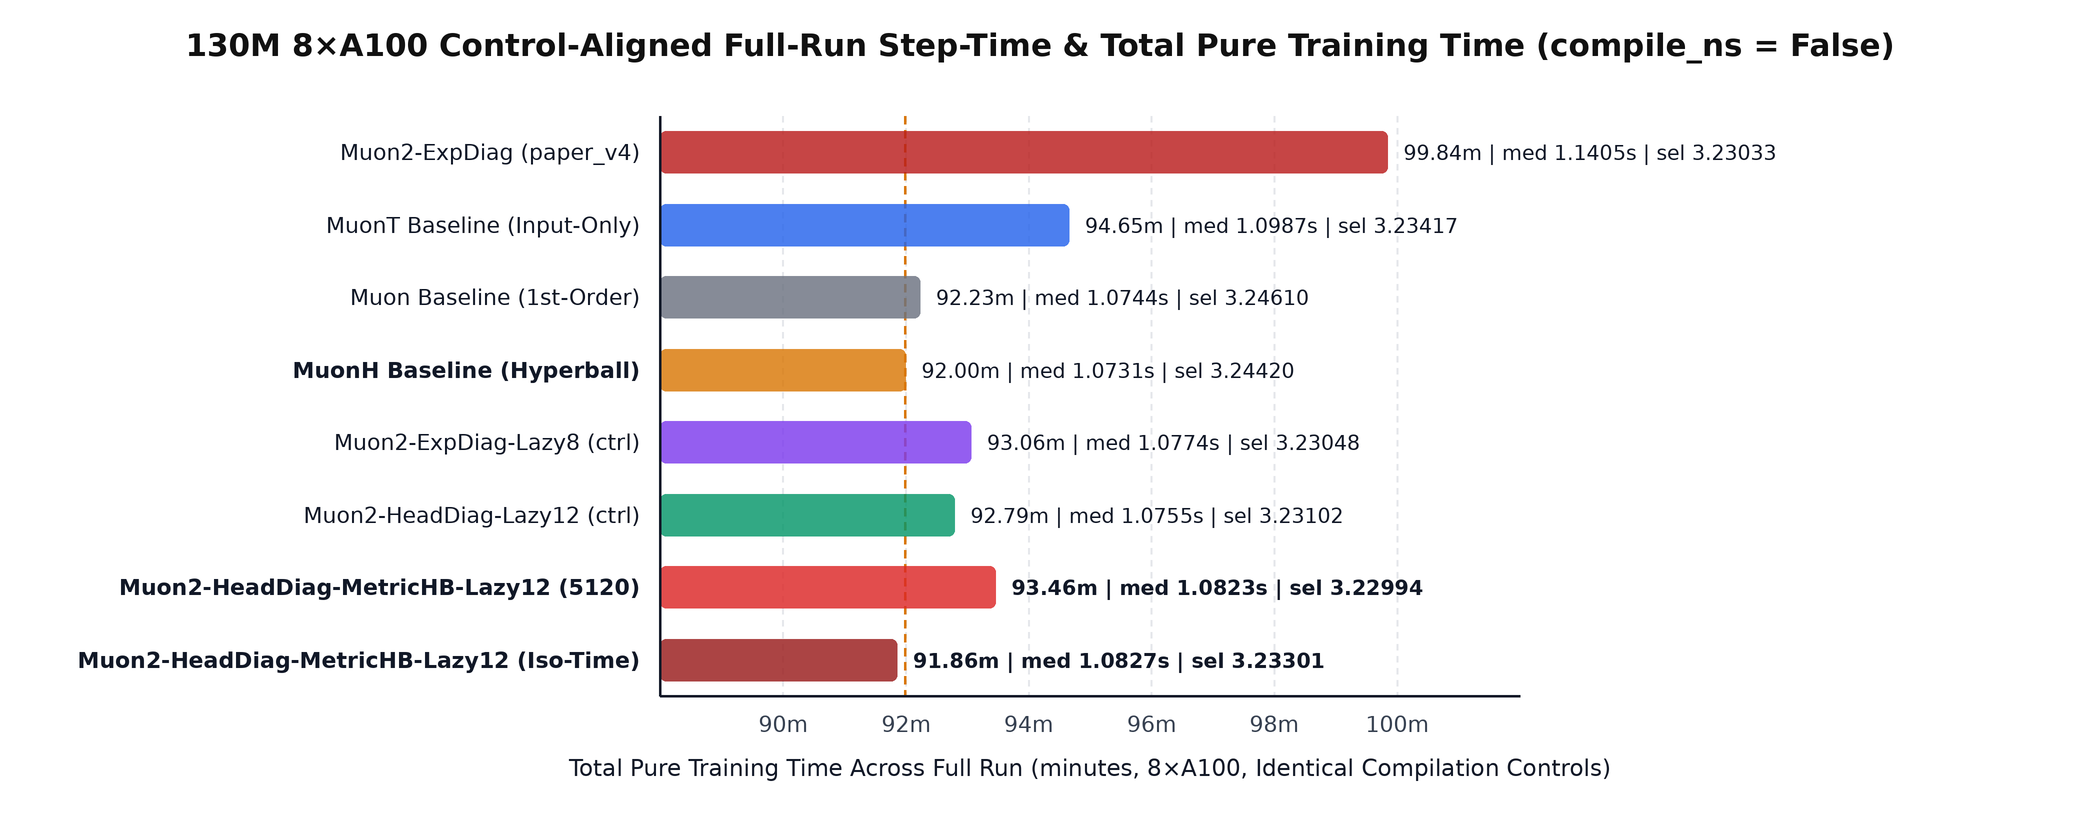
\includegraphics[width=0.96\textwidth]{step_time_waterfall_130m_eff.png}
\caption{Full-run pure training time and steady-state median step time across strictly control-aligned 130M runs (\texttt{compile\_ns = False}, $8\times\text{A100}$). Lazy capture + dual-sided async-host roots eliminate $\approx 89\text{--}95\%$ of \texttt{paper\_v4}'s overhead; the $5{,}030$-step iso-time schedule finishes strictly faster ($91.86\text{m}$) than both \mname{MuonH} ($92.00\text{m}$) and \mname{Muon} ($92.23\text{m}$).}
\label{fig:waterfall}
\end{figure}

\section{Empirical Results at 130M (\texorpdfstring{1$\times$}{1x} Chinchilla, 2.68B Tokens)}
\label{sec:results}

\subsection{Component-by-Component Ablation and Strict Iso-Time Verification (Seed 0)}

\Cref{tab:seed0,fig:waterfall,fig:seed0} trace each component under identical compilation controls (\texttt{compile\_ns = False}):
\begin{itemize}
  \item \textbf{Pure systems \& cadence speedup (\mname{ExpDiag-Lazy8}):} Keeping \texttt{paper\_v4}'s exact factor placement (\texttt{q,k,v,o,down} Dense, \texttt{gate,up} Diag, $Q = W\hat{R}^2$) while switching to $K = 8$ single-microbatch capture + dual-sided async-host roots cuts pure training time from $99.84\text{m}$ to $\mathbf{93.06\text{m}}$ ($-6.78\text{m}$) with identical final quality ($\Lsel = 3.23048$ vs.\ $3.23033$, $\Lc = 3.44683$ vs.\ $3.44720$), flipping \mname{Muon2-ExpDiag}'s $+23.5\times 10^{-3}$ nat deficit at \mname{MuonH}'s $92.0\text{m}$ finish into a $\mathbf{-10.8\times 10^{-3}}$ nat lead.
  \item \textbf{Per-head \texttt{q,k} structure (\mname{HeadQK-Lazy12}):} Switching \texttt{q,k} to $8\times 64\times 64$ per-head blocks at $K = 12$ lowers median step time to $\mathbf{1.0755\text{s}}$ ($+1.1\text{ ms}$ / $+0.10\%$ vs.\ \mname{Muon}'s $1.0744\text{s}$; $92.79\text{m}$ total) at $\Lpal = 3.39899$.
  \item \textbf{Right-Metric Tangential Hyperball (\mname{HeadQK-MetricHB-Lazy12}):} Adding \mname{MetricHB} slashes \texttt{Late-11} loss by $-9.9\times 10^{-3}$ nats ($3.34515$ vs.\ $3.35506$, and $-15.1\times 10^{-3}$ vs.\ \mname{MuonH}'s $3.36025$) while achieving the best overall Seed-0 $\Lsel = \mathbf{3.22994}$, $\Lc = \mathbf{3.44601}$, and 16-domain $\Lpal = \mathbf{3.39816}$. Truncating its WSD schedule to $5{,}030$ steps (\textbf{Iso-Time}, $91.86\text{m} < 92.00\text{m}$ \mname{MuonH}) still completes full cooldown $\mathbf{-11.19\times 10^{-3}}$ nats below \mname{MuonH} and $\mathbf{-13.09\times 10^{-3}}$ nats below \mname{Muon}.
\end{itemize}

\begin{table}[t]
\centering
\caption{Seed-0 component ablations and strict iso-time verification under identical compilation controls (\texttt{compile\_ns = False}, $8\times\text{A100}$). $\Lsel\text{ @ }92.0\text{m}$ evaluates each curve at \mname{MuonH}'s exact completion time.}
\label{tab:seed0}
\resizebox{\textwidth}{!}{%
\begin{tabular}{@{}lrrrrrrr@{}}
\toprule
Method (Seed 0, \texttt{compile\_ns = False}) & Steps & Pure Time & Med Step & $\Lsel$ @ $92.0\text{m}$ & Final $\Lsel$ & Final $\Lc$ & $\Lpal$ (16-Dom.) \\
\midrule
\mname{Muon} ($\eta = 0.016$) & $5{,}120$ & $92.23\text{m}$ & $1.0744\text{s}$ & $3.24689$ & $3.24610$ & $3.46181$ & --- \\
\mname{MuonH} ($\eta = 0.01131$) & $5{,}120$ & $92.00\text{m}$ & $1.0731\text{s}$ & $3.24420$ & $3.24420$ & $3.46145$ & $3.41605$ \\
\mname{MuonT} ($\eta = 0.016$) & $5{,}120$ & $94.65\text{m}$ & $1.0987\text{s}$ & $3.24296$ & $3.23417$ & $3.45106$ & $3.40407$ \\
\mname{Muon2-ExpDiag} (\texttt{paper\_v4}, $K=1$) & $5{,}120$ & $99.84\text{m}$ & $1.1405\text{s}$ & $3.26770$ & $3.23033$ & $3.44720$ & $3.39854$ \\
\midrule
\mname{ExpDiag-Lazy8} ($Q = W\hat{R}^2$, $K=8$) & $5{,}120$ & $93.06\text{m}$ & $1.0774\text{s}$ & $3.23340$ & $3.23048$ & $3.44683$ & $3.39887$ \\
\mname{HeadQK-Lazy12} ($Q = W\hat{R}^2$, $K=12$) & $5{,}120$ & $\mathbf{92.79\text{m}}$ & $\mathbf{1.0755\text{s}}$ & $3.23326$ & $3.23102$ & $3.44745$ & $3.39899$ \\
\rowcolor{ourstint}
\textbf{\mname{HeadQK-MetricHB-Lazy12} (Iso-Time)} & $\mathbf{5{,}030}$ & $\mathbf{91.86\text{m}}$ & $1.0827\text{s}$ & $3.23301$ & $3.23301$ & $3.44968$ & $3.40415$ \\
\rowcolor{ourstint}
\textbf{\mname{HeadQK-MetricHB-Lazy12} (Full, Ours)} & $\mathbf{5{,}120}$ & $93.46\text{m}$ & $1.0823\text{s}$ & $\mathbf{3.23294}$ & $\mathbf{3.22994}$ & $\mathbf{3.44601}$ & $\mathbf{3.39816}$ \\
\bottomrule
\end{tabular}%
}
\end{table}

\begin{figure}[t]
\centering
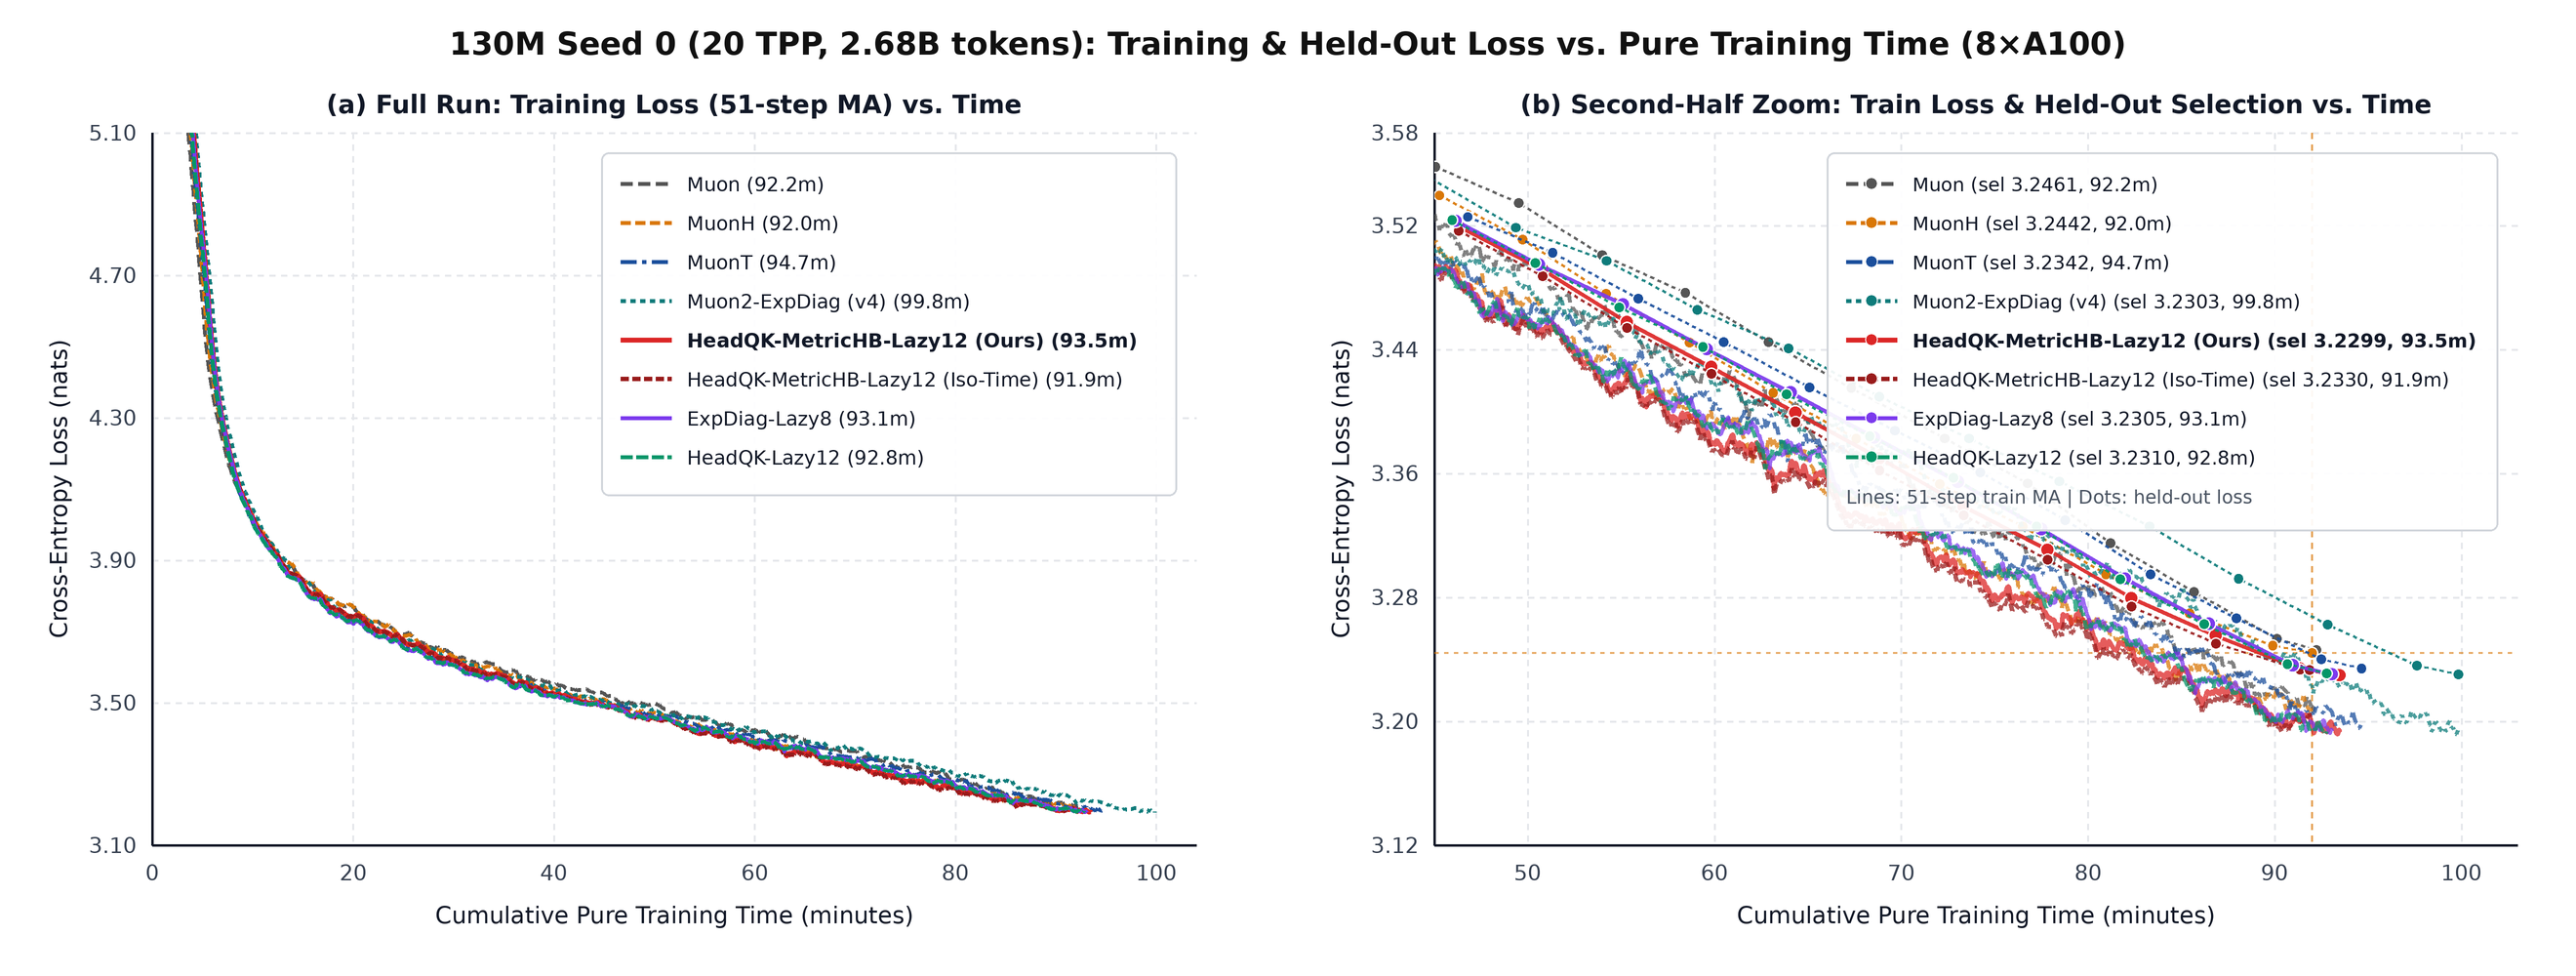
\includegraphics[width=\textwidth]{training_loss_vs_time_130m_seed0_eff.png}
\caption{Seed-0 training loss ($51$-step MA) and held-out selection loss vs.\ cumulative pure training time ($8\times\text{A100}$, \texttt{compile\_ns = False}). Vertical/horizontal orange dashed guides mark \mname{MuonH}'s finish ($92.0\text{m}$, $\Lsel = 3.2442$).}
\label{fig:seed0}
\end{figure}

\subsection{Paired Fresh Multi-Seed Confirmation (Seeds 1, 2, 3)}

\Cref{tab:seeds,tab:isotime_ms,fig:seeds123} report replication on three untouched paired seeds (\texttt{Seeds 1, 2, 3}):
\begin{itemize}
  \item \textbf{Final and out-of-distribution quality (\cref{tab:seeds}):} \mname{HeadQK-MetricHB-Lazy12} achieves $\Lsel = \mathbf{3.18714 \pm 0.0279}$ ($\mathbf{-16.40 \pm 1.29}\times 10^{-3}$ nats vs.\ \mname{Muon}, $\mathbf{-15.41 \pm 1.23}\times 10^{-3}$ nats vs.\ \mname{MuonH}, $-4.49\times 10^{-3}$ vs.\ \mname{MuonT}, $-5.13\times 10^{-3}$ vs.\ \mname{MuonTH}, $-3.36\times 10^{-3}$ vs.\ Euclidean \mname{Muon2-ExpDiagH}, and $-0.99\times 10^{-3}$ nats ahead of \texttt{paper\_v4}'s \mname{Muon2-ExpDiag} while saving $6.86\text{ minutes}$ per run). On 16-domain Paloma, it beats both \mname{Muon} ($-14.16\times 10^{-3}$) and \mname{MuonH} ($-13.62\times 10^{-3}$) on \textbf{$19/19$ evaluated domain splits}.
  \item \textbf{Uniform wall-clock dominance (\cref{tab:isotime_ms}):} Unlike $Q = W\hat{R}^2$ methods that trail \mname{MuonH} mid-run, \mname{HeadQK-MetricHB-Lazy12} stays $\mathbf{-8.8}$ to $\mathbf{-16.4\times 10^{-3}}$ \textbf{nats below \mname{MuonH} at every wall-clock minute} from $t = 40\text{m}$ through \mname{Muon}/\mname{MuonH}'s $92.01\text{m}$ finish ($\mathbf{3.18927}$ vs.\ $3.20255$, a $\mathbf{-13.28\times 10^{-3}}$ nat equal-compute lead).
\end{itemize}

\begin{table}[t]
\centering
\caption{Paired fresh \texttt{Seeds 1, 2, 3} confirmation at 130M ($5{,}120$ steps $= 2.68\text{B}$ tokens, \texttt{compile\_ns = False}). Paired $\Delta$ values are reported in $10^{-3}$ nats ($\text{mean} \pm \text{SD}$ across paired seeds; negative favors our method).}
\label{tab:seeds}
\resizebox{\textwidth}{!}{%
\begin{tabular}{@{}lrrrrrrrr@{}}
\toprule
Method (\texttt{Seeds 1--3}) & Pure Time & Med Step & Held-Out $\Lsel$ & $\Delta\Lsel$ vs.\ \mname{Muon} & $\Delta\Lsel$ vs.\ \mname{MuonH} & C4 $\Lc$ & Late-11 & Paloma $\Lpal$ \\
\midrule
\mname{Muon} ($\eta=0.016$) & $92.01\text{m}$ & $1.0744\text{s}$ & $3.20354 \pm .0289$ & $0.00$ & $+0.99$ & $3.46404$ & $3.33753$ & $3.41641$ \\
\mname{MuonH} ($\eta=0.01131$) & $92.04\text{m}$ & $1.0747\text{s}$ & $3.20255 \pm .0291$ & $-0.99 \pm 0.72$ & $0.00$ & $3.46262$ & $3.31630$ & $3.41587$ \\
\mname{MuonT} ($\eta=0.016$) & $94.35\text{m}$ & $1.0957\text{s}$ & $3.19163 \pm .0302$ & $-11.91 \pm 1.56$ & $-10.92$ & $3.45225$ & $3.31427$ & $3.40491$ \\
\mname{MuonTH} ($\eta=0.01131$) & $94.80\text{m}$ & $1.1005\text{s}$ & $3.19227 \pm .0291$ & $-11.27 \pm 0.42$ & $-10.28$ & $3.45419$ & $3.30471$ & $3.40416$ \\
\mname{Muon2-ExpDiag} (\texttt{v4}) & $100.00\text{m}$ & $1.1412\text{s}$ & $3.18813 \pm .0306$ & $-15.41 \pm 1.88$ & $-14.42$ & $3.44840$ & $3.31074$ & $\mathbf{3.40050}$ \\
\mname{Muon2-ExpDiagH} & $99.25\text{m}$ & $1.1372\text{s}$ & $3.19050 \pm .0282$ & $-13.04 \pm 0.77$ & $-12.05$ & $3.45137$ & $3.30161$ & $3.40293$ \\
\rowcolor{ourstint}
\textbf{\mname{HeadQK-MetricHB-Lazy12}} & $\mathbf{93.14\text{m}}$ & $\mathbf{1.0790\text{s}}$ & $\mathbf{3.18714 \pm .0279}$ & $\mathbf{-16.40 \pm 1.29}$ & $\mathbf{-15.41 \pm 1.23}$ & $\mathbf{3.44741}$ & $\mathbf{3.30029}$ & $3.40225$ \\
\bottomrule
\end{tabular}%
}
\end{table}

\begin{table}[t]
\centering
\caption{Mean held-out selection loss $\Lsel(t)$ across paired \texttt{Seeds 1--3} interpolated at matched pure wall-clock training minutes $t \in [40, 92.01]$ (\texttt{compile\_ns = False}).}
\label{tab:isotime_ms}
\resizebox{\textwidth}{!}{%
\begin{tabular}{@{}rrrrrrr@{}}
\toprule
Wall-Clock Time $t$ & \mname{Muon} & \mname{MuonH} & \mname{MuonT} & \mname{Muon2-ExpDiag} (\texttt{v4}) & \textbf{\mname{HeadQK-MetricHB-Lazy12}} & \textbf{Lead vs.\ \mname{MuonH}} \\
\midrule
$40.00\text{m}$ & $3.55619$ & $3.54100$ & $3.52904$ & $3.54164$ {\footnotesize($+0.64$)} & $\mathbf{3.52463}$ & $\mathbf{-16.37\times 10^{-3}}$ \\
$50.00\text{m}$ & $3.48721$ & $3.46263$ & $3.45972$ & $3.47668$ {\footnotesize($+14.05$)} & $\mathbf{3.45090}$ & $\mathbf{-11.73\times 10^{-3}}$ \\
$60.00\text{m}$ & $3.42056$ & $3.39011$ & $3.40097$ & $3.41860$ {\footnotesize($+28.49$)} & $\mathbf{3.37939}$ & $\mathbf{-10.72\times 10^{-3}}$ \\
$70.00\text{m}$ & $3.35102$ & $3.32260$ & $3.33837$ & $3.36222$ {\footnotesize($+39.62$)} & $\mathbf{3.31301}$ & $\mathbf{-9.59\times 10^{-3}}$ \\
$80.00\text{m}$ & $3.27940$ & $3.25856$ & $3.27528$ & $3.30147$ {\footnotesize($+42.91$)} & $\mathbf{3.24978}$ & $\mathbf{-8.78\times 10^{-3}}$ \\
$90.00\text{m}$ & $3.21014$ & $3.20694$ & $3.21010$ & $3.23796$ {\footnotesize($+31.02$)} & $\mathbf{3.19583}$ & $\mathbf{-11.11\times 10^{-3}}$ \\
\rowcolor{ourstint}
$\mathbf{92.01\text{m}}$ {\footnotesize(\mname{Muon} end)} & $3.20354$ & $3.20255$ & $3.19867$ & $3.22560$ {\footnotesize($+23.05$)} & $\mathbf{3.18927}$ & $\mathbf{-13.28\times 10^{-3}}$ \\
\bottomrule
\end{tabular}%
}
\end{table}

\begin{figure}[t]
\centering
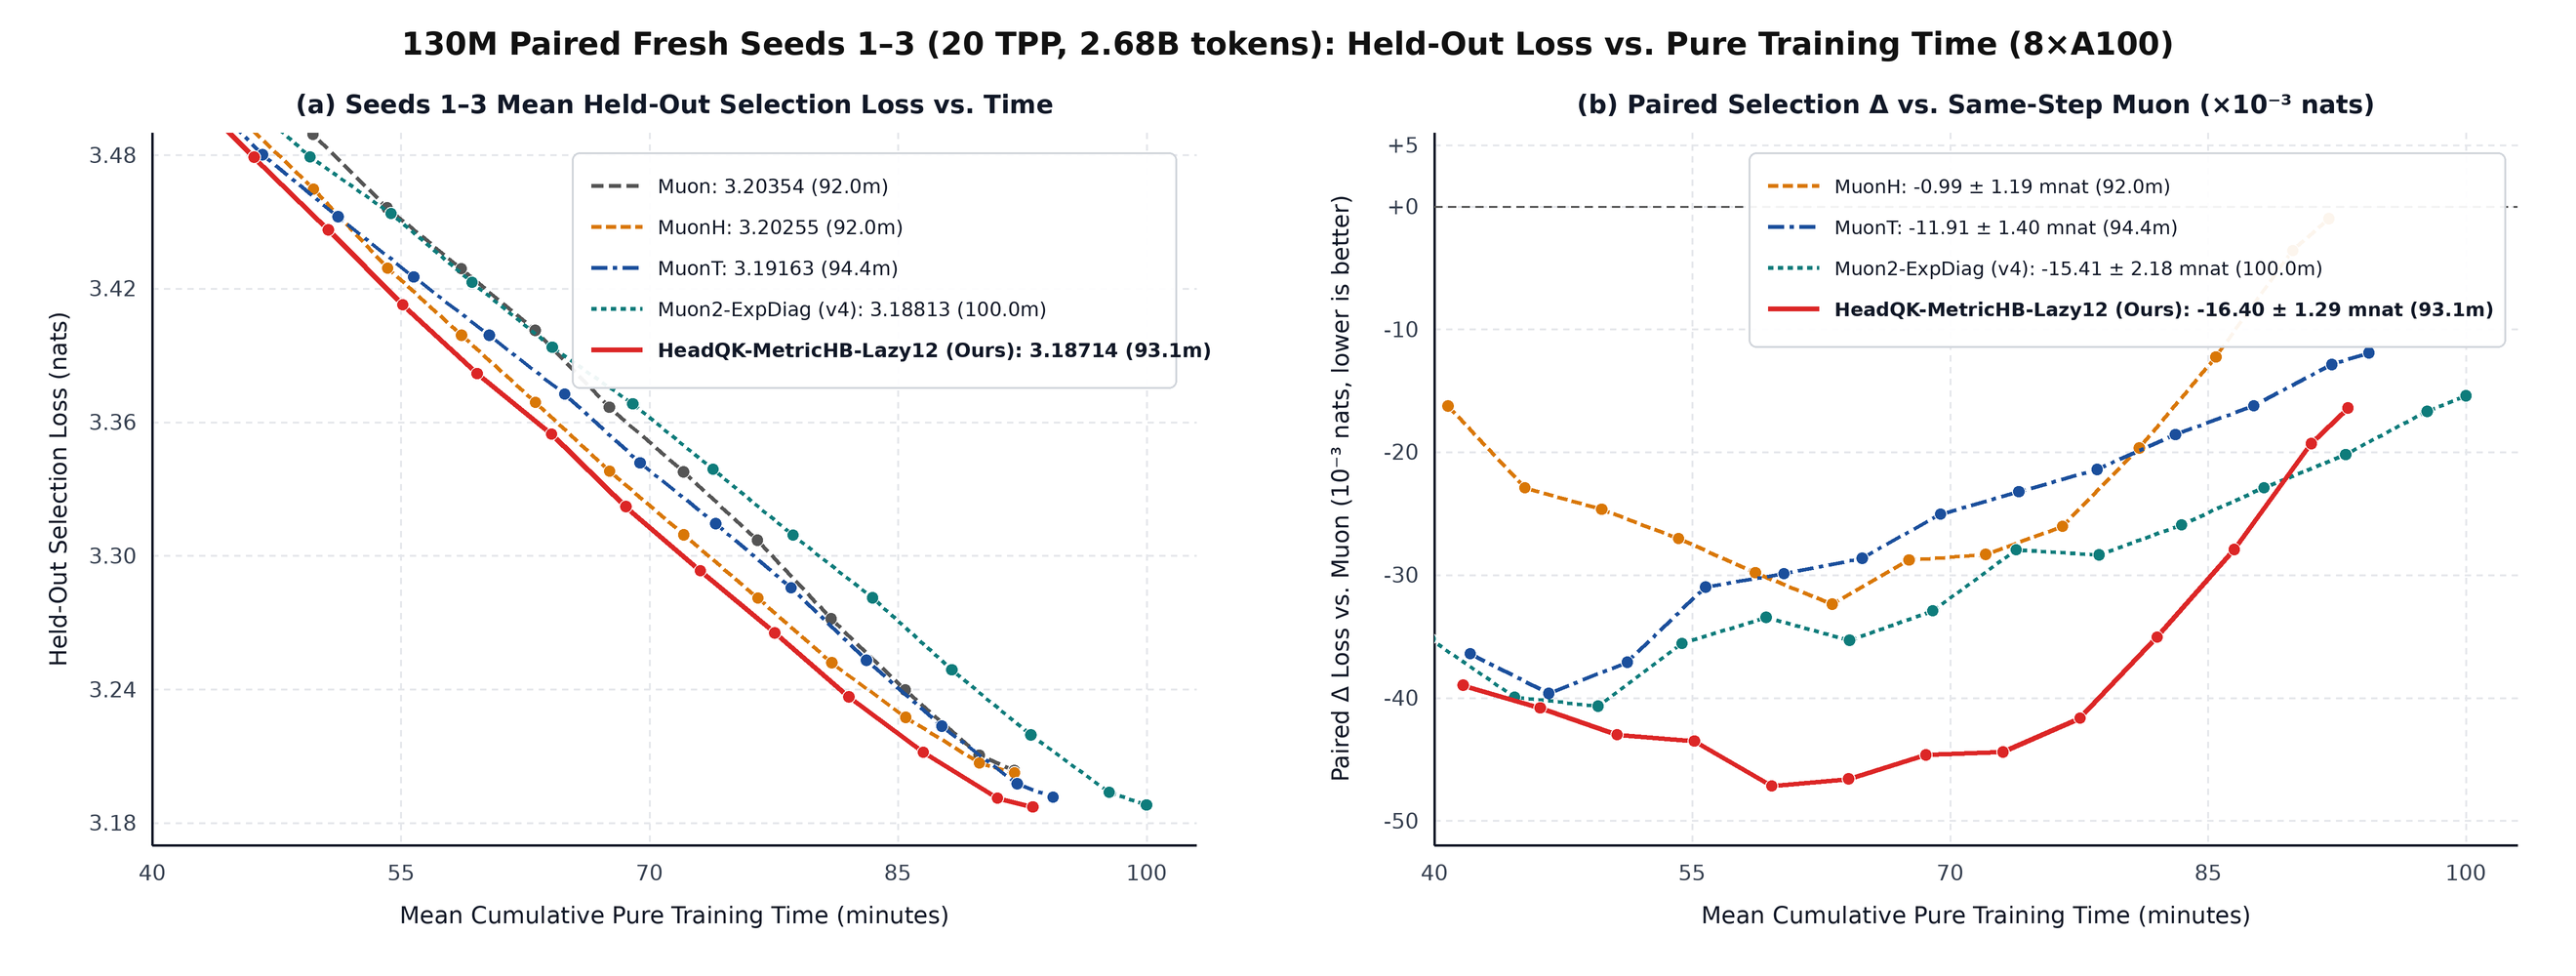
\includegraphics[width=\textwidth]{training_loss_vs_time_130m_seeds123_eff.png}
\caption{Paired fresh \texttt{Seeds 1--3}: (a)~mean held-out selection loss vs.\ pure training time; (b)~paired difference vs.\ same-step \mname{Muon} plotted against each method's own cumulative pure training time.}
\label{fig:seeds123}
\end{figure}

\FloatBarrier
\section{Summary of Recommendations}
\label{sec:conclusion}

\begin{enumerate}
  \item \textbf{Drop-in decoupled-decay recipe (\mname{HeadQK-Lazy12}):} When keeping standard decoupled $Q = W\hat{R}_t^2$ ($\eta = 0.016, \lambda = 0.1$) is desired, $K = 12$ single-microbatch capture + dual-sided async-host exact roots + $8\times 64^2$ per-head \texttt{q,k} blocks reduces median step-time overhead vs.\ \mname{Muon} to $+0.10\%$ ($92.79\text{m}$ vs.\ $92.23\text{m}$) with full \mname{Muon2-ExpDiag} accuracy.
  \item \textbf{Default wall-clock Pareto recipe (\mname{HeadQK-MetricHB-Lazy12}):} Pairing \mname{HeadQK-Lazy12} with Right-Metric Tangential Hyperball (\cref{eq:metrichb}, $\eta = 0.01345, \lambda = 0.15$) dominates \mname{Muon}, \mname{MuonH}, \mname{MuonT}, and \mname{Muon2-ExpDiag} across \emph{every} wall-clock training budget ($40\text{m}$ through $93\text{m}$) at $+0.43\%$ median step overhead.
\end{enumerate}

\end{document}
